%\documentclass[11pt,a4paper]{article}
\documentclass[11pt,a4paper]{book}
\usepackage[english]{babel}
\usepackage{graphicx,latexsym,isabelle,isabellesym,pdfsetup}

% proper setup for best-style documents
\urlstyle{rm}
\isabellestyle{it}

\pagestyle{myheadings}

%make a bit more space
\addtolength{\hoffset}{-1,5cm}
\addtolength{\textwidth}{3cm}
\addtolength{\voffset}{-1cm}
\addtolength{\textheight}{2cm}

\newcommand{\secref}[1]{Section~\ref{#1}}
\newcommand{\secrefs}[1]{Sections~\ref{#1}}
\newcommand{\charef}[1]{Chapter~\ref{#1}}
\newcommand{\charefs}[1]{Chapters~\ref{#1}}

%remove clutter from the toc
\setcounter{secnumdepth}{2}
\setcounter{tocdepth}{1}

\begin{document}

\title{Jinja with Threads}
\author{Andreas Lochbihler}
\maketitle

\begin{trivlist}
\item \textbf{Abstract.}
  We extend the Jinja source code semantics by Klein and Nipkow with Java-style arrays and threads.
  Concurrency is captured in a generic framework semantics for adding concurrency through interleaving to a sequential semantics, which features dynamic thread creation, inter-thread communication via shared memory, lock synchronisation and joins. Also, threads can suspend themselves and be notified by others.
  We instantiate the framework with the adapted versions of both Jinja source and byte code and show type safety for the multithreaded case. 
  Equally, the compiler from source to byte code is extended, for which we prove weak bisimilarity between the source code small step semantics and the defensive Jinja virtual machine.
  On top of this, we formalise the JMM and show the DRF guarantee and consistency.

  For description of the different parts, see \cite{Lochbihler2008FOOL,Lochbihler2010ESOP,LochbihlerBulwahn2011ITP,Lochbihler2012ESOP}.
\end{trivlist}

\tableofcontents

%\section{Theory Dependencies}

%Figure \ref{theory-deps} shows the dependencies between 
%the Isabelle theories in the following sections.

%\begin{figure}[h!t]
%\begin{center}
%  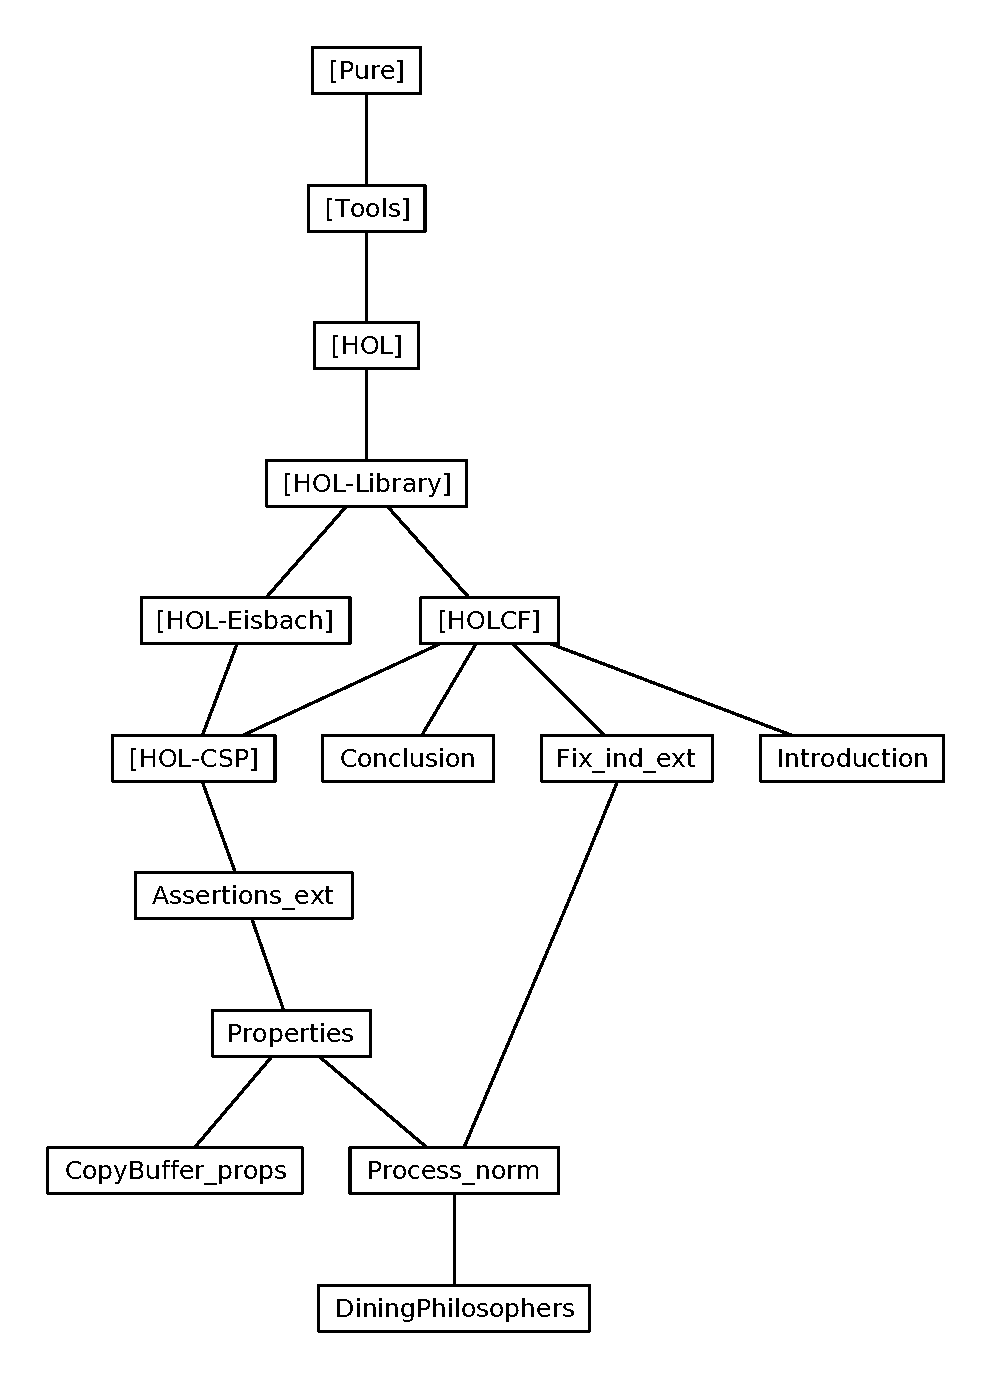
\includegraphics[height=\textheight]{session_graph}
%\end{center}
%\caption{Theory Dependency Graph\label{theory-deps}}
%\end{figure}

\clearpage

\input{session}

\bibliographystyle{plain}
\bibliography{root}

\end{document}
